\documentclass[12pt,a4paper]{report}
\usepackage[hmargin=3cm,vmargin=3cm]{geometry}
\usepackage{graphicx}
\usepackage{caption}
\usepackage{array}
\usepackage{listings}
\usepackage{hyperref}
\usepackage{mathtools}
\usepackage{textcomp}
\usepackage{amsmath}
\usepackage{float}
\graphicspath{Images}
\begin{document}
\begin{figure}
\centering

\includegraphics[width = 0.3\textwidth]{iit.png}
\hspace{1cm}

\includegraphics[width = 0.4\textwidth]{fossee-logo.png}
\end{figure}

\title{\textbf{\textbf{Summer Fellowship Report}}\vspace{3mm} \\\small On \\\vspace{3mm} \textbf{\large FOSSEE Scilab Signal Processing Toolbox and\\ Communication Toolbox}\vspace{3mm} \\ \vspace{3mm}\small Submitted by\\  \vspace{3mm}  \large \textbf{Y Shashi Kiran}\\ \vspace{2mm}  \large \textbf{Kartik Vishnu Hegde}\\ \vspace{2mm}  \large \textbf{Sonu Sharma}\\ \vspace{7mm}
\small Under the guidance of \\  \vspace{3mm}
\large \textbf{Prof. Kannan M Moudgalya} \vspace{1mm}\\
\large \textbf{Prof. Kumar Appaiah} \vspace{5 mm}\\
\small Mentors
\\ 
\vspace{1mm} \large \textbf{Mr Rupak Rokade}\\ 
\vspace{1mm}  \large \textbf{Mr Sudhakar Kumar}\\  
}

\maketitle


\title{\textbf{\textbf{\LARGE 
\begin{flushleft}
\textbf{Acknowledgment}
\end{flushleft}
}}}
\large \hspace{1.5cm}   The internship opportunity we had with the FOSSEE Team,\\IIT BOMBAY, was a great chance for learning and professional development. Therefore, we consider ourselves as very lucky individuals as we were provided with an opportunity to be a part of it. We are also grateful for having a chance to meet so many wonderful people and professionals across the country who led us through this internship period.\\
We are using this opportunity to express our deepest gratitude and special thanks to Prof. Kannan M Moudgalya, head of FOSSEE team, IIT Bombay, for giving us an opportunity to be a part of this project.\\
We express our deepest thanks to Prof. Kumar Appaiah, professor in the Department of Electrical Engineering, IIT Bombay, for taking part in useful decisions and giving necessary advices and guidance to make life easier. We choose this moment to acknowledge his contribution gratefully.\\
It is our radiant sentiment to place on record our best regards, deepest sense of gratitude to our mentors, Mr Rupak Rokade and Mr Sudhakar Kumar for their continuous support which were extremely valuable for our study both theoretically and practically and helping us to learn a lot many things.\\\\
We perceive this opportunity as a big milestone in our career development. We will strive to use gained skills and knowledge in the best possible way, and we will continue to work on their improvement, in order to attain desired career objectives. Hope to continue cooperation with all of you in the future.


\tableofcontents

\chapter{\textbf{Introduction}}

\section{About Scilab Signal Processing Toolbox}
The Scilab Signal Processing toolbox that we are working on has around 280 functionalities. We had been given a task of fixing and developing around 85 functions of the toolbox. 
This toolbox tries to match the toolbox of same kind in other computational softwares like Octave or MATLAB in almost all of the cases. There are few exceptions in Scilab ,for example, the function \char`\"filter\char`\" in scilab accepts only real vectors or matrices as input arguments but not so in the case of MATLAB and Octave. But these limitations on the output are seen quite less and we have worked on it, seeing to that the values are matched. \\
\\
The toolbox has algorithms with highly diverse complexities in the implementations. There are algorithms ranging from simple implementation of windows to complex signal processing algorithms like MUSIC( pmusic and rootmusic ) algorithms,fir1,fir2 and icceps.
\\
\\
Almost fifteen windows necessary for signal processing have been added to the toolbox.\\
We have also added all the necessary documents and help files for each and every functions that we have worked on.\\
So ,Scilab being an open source software, most of the signal processing algorithms that are implemented in MATLAB can be implemented easily for free using our toolbox.  


\section{git}
Git is a version control system for tracking changes happening in files of computer, Git along with web based hosting services for repository (like GitHub, ) can be used to coordinating work among multiple people across the world.\\
We have made the toolbox in our systems as git repositories(local repository) to push it to github (to create a remote repository).

\begin{figure}[H]
\centering
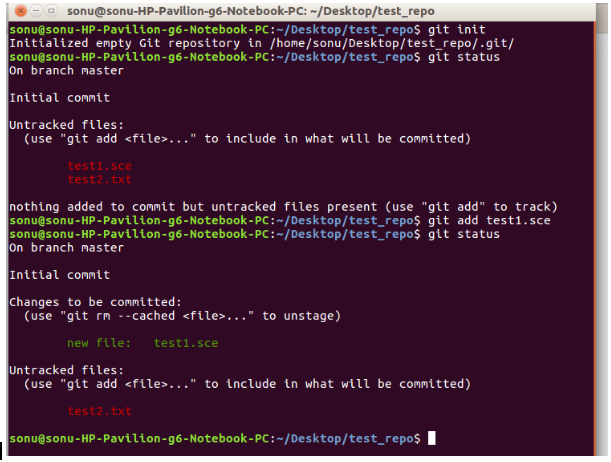
\includegraphics[width = 0.8\textwidth]{git.png}
\captionof{figure}{ git commands}
\label{gitcommand}
\end{figure}


The figure\ref{gitcommand} shows the process of initializing local git repository.

\section{GitHub}

GitHub is a web-based hosting service for version control using Git.  It is mostly used for computer code. It offers all of the distributed version control and source code management (SCM) functionality of Git as well as adding its own features.\\

We have used github for version control using Git.And we used github for one more major purpose that is linking it with Travis CI , the continuous integration tool , where we can deploy and test our projects which are in the github. The file \char`\".travis.yml\char`\" in github indicates the Travis CI to test our projects. ( See section 2.2.2)\\


\section{Travis CI}
Travis is a continuous integration tool , where we can deploy and test our projects which are in the github. We linked our github repository to our travis CI account and then we initiated a build in travis.\\

Travis just looks into the .travis.yml file in the repository , and based on the script that we have mentioned , it builds our project.\\

\begin{figure}[H]
\centering
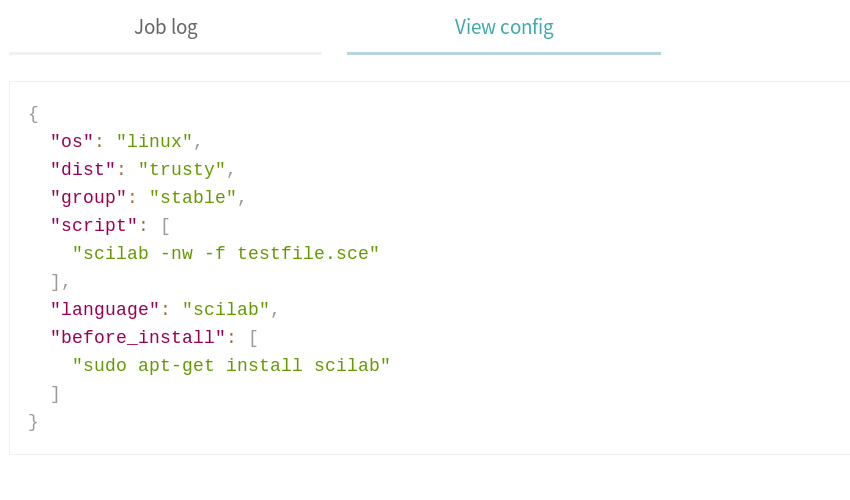
\includegraphics[width = 0.8\textwidth]{travisconfig.png}
\captionof{figure}{The basic configuration of the travis engine }
\label{travisci}
\end{figure}
The figure\ref{travisci} shows the basic configuratrion of Travis CI Engine.\\

We basically build the testfile.sce of the toolbox in Travis CI, which is used to validate the functions present in the toolbox. \\
As seen in .travis.yml file, commands:\\
    sudo apt-get install scilab      ……...installs scilab in travis engine\\
    scilab -nw -f testfile.sce         ……...executes testfile.sce in a scilab window on the terminal without gui.\\\\

On successful completion of the build we get an indication as shown:\\
\begin{figure}[H]
\centering
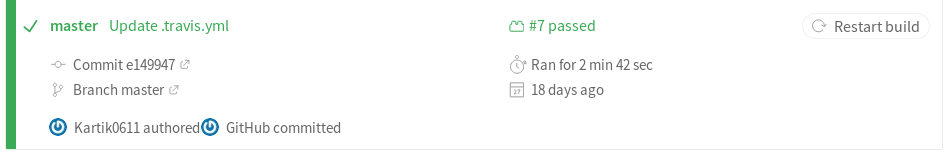
\includegraphics[width = 0.8\textwidth]{travissuccess.png}
\captionof{figure}{Successful build on travis}
\end{figure}


If the build fails, then we get an indication as follows:\\
\begin{figure}[H]
\centering
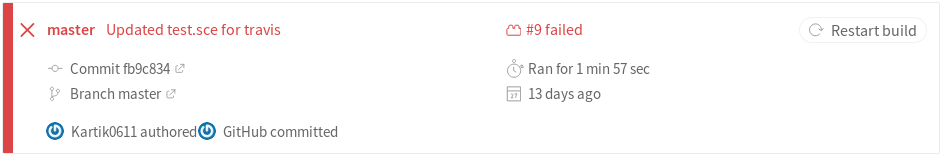
\includegraphics[width = 0.8\textwidth]{travisfail.png}
\captionof{figure}{Failure of a build in travis}
\end{figure}
It indicates that we have to revisit the testfile to fix the errors or bugs.\\
After each and every build, be it successful or failed builds, we get notification mails from travis regarding the commit information and the build status.\\
So each time, we triggered the builds by the entering the desired commit messages of the git repository, to test the toolbox.

\newpage













\chapter{\textbf{Structure of the Signal Processing toolbox}}
The toolbox has two types of files:
\section{Visible Files}
\begin{itemize}
\item loader.sce
\item builder.sce
\item demos
\item etc
\item jar
\item cleaner.sce
\item testfile.sce
\item unloader.sce
\item README.md
\item help
\end{itemize}

The primary step that one has to do, to use this toolbox for the first time is that , one has to essentially go through the README.md file of the toolbox. This file has the text providing the guidance on how to use the toolbox.  

\subsection{loader.sce}
It’s basically a file that calls for the function FOSSEE\textunderscore Signal\textunderscore processing\textunderscore toolbox.start present in the etc folder. This has to be executed first on opening the toolbox, using the command \char`\"exec loader.sce\char`\".
in the scilab console.


\subsection{builder.sce}
This file builds the macros,help and the loader.sce files. Type the command \char`\"exec builder.sce\char`\" in the scilab console to execute this file.\\
Both these have to executed every time, to load the toolbox for usage.

\subsection{demos}
This folder includes the examples taken from  \url{https://in.mathworks.com/help/signal/examples/dft-estimation-with-the-goertzel-algorithm.html }, which is function used for DFT Estimation with the Goertzel Algorithm.

\subsection{macros}
It’s the main folder of the toolbox, which has all the signal processing functions of the toolbox.

\subsection{etc}
Its a folder which consists of FOSSEE\textunderscore Signal\textunderscore processing\textunderscore toolbox.start and FOSSEE\textunderscore Signal\textunderscore processing\textunderscore toolbox.quit files.
These files are used to start and exit files of the toolbox.

.start file
It will run a script when loader.sce is run from root toolbox directory. It will run loader files in all of the directories and link to important library.

.quit file
It will run a script when unloader.sce is run from root toolbox directory. It will unlink all of the important libraries.


\subsection{jar}
This folder has scilab\textunderscore en\textunderscore US.jar file. This file is basically a Java Archive package file format typically used to aggregate many Java class files and associated metadata and resources (text,images etc.) into a file for distribution.

\subsection{cleaner.sce}
This file is generated by builder.sce. On executing this file, we actually delete the loader.sce and the unloader.sce files.
One caution to the users is that  \textbf{do not edit this file.}

\subsection{testfile.sce}
This file is used to validate all the functions present in the toolbox macros. This file is executed in the Travis CI (Continuous Integration).

\subsection{unloader}
It unloads the toolbox.

\subsection{help}
It contains the help files of all the functions present in the toolbox(macros) as .xml files.

\section{Hidden Files}
These files have to included in the git repository before pushing it to the github. To view these files in the git repository use the command:  \\
\char`\"ls -a\char`\"   on the terminal in the git repository directory.  


\begin{itemize}
\item .gitignore 
\item .travis.yml
\end{itemize}

\subsection{.gitignore}
This file enables the user to explicitly tell git to ignore certain files. In our toolbox, we have included just a statement  \char`\" \char`\* \char`\~ \char`\" , indicating that all the file names having the sign \char`\"\char`\~\char`\" (\char`\"tilde\char`\") in the end(or suffixed) are ignored by git (when intentionally gone untracked).  

\subsection{.travis.yml}
This file is included to facilitate the builds we can trigger in Travis CI. \\
Travis CI actually provides a default build environment and a default set of steps for each programming language. We can customize any step in this process in .travis.yml. Travis CI uses .travis.yml file in the root of our repository to learn about our project and how we want our builds to be executed. .travis.yml can be very minimalistic or have a lot of customization in it.

\begin{figure}[H]
\centering
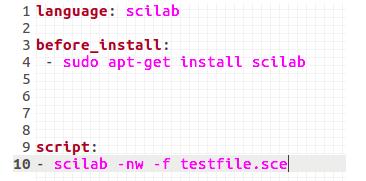
\includegraphics[width = 0.5\textwidth]{travisyml.png}
\captionof{figure}{ .travis.yml file}
\end{figure}

The above figure shows the different sections involved in the .travis.yml file.\\
So each time when a build is triggered by the user, tracis engine actually downloads scilab (as per before\textunderscore install section) and then a new scilab instance is opened in the terminal without any gui (-nw flag) and executes testfile.sce in the toolbox ( because of the -f flag used here).

\chapter{\textbf{Our Work}}
                   
The toolbox mainly had issues with around 85 functions which were given to us like a problem statement by our mentors to debug. These functions were of two kinds:\\


\begin{itemize}
\item Functions built in Scilab
\item Functions using Scilab Octave Interface Toolbox\\
\end{itemize}

The issues with the functions built in Scilab were fixed and every function was added with required documentation , help files and test cases. We have also worked on adding plots in the help files. We have also added equations and matrices in the help files using LaTeX.\\
Few functions ,of such kind, we worked on are shown below:\\
Example 1:\\
\textbf{Medfilt1} : Function for 1D median filtering\\
Description\\
y = medfilt1(x)\\
Applies a 3rd order 1-dimensional median filter to input x along the first non-zero dimension.\\
The function appropriately pads the signal with zeros at the endings. For a segment, a median is calculated as the middle value (average of two middle values) for odd number number (even number) of data points.\\
\begin{figure}[H]
\centering
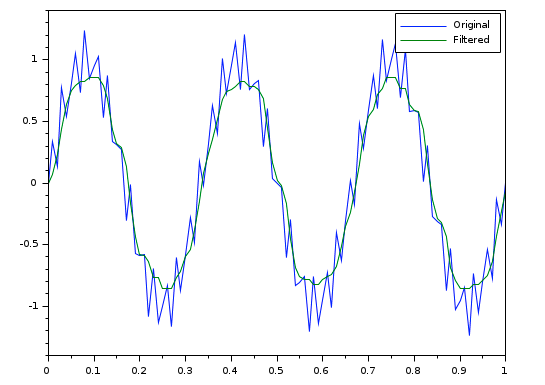
\includegraphics[width = 0.6\textwidth]{medfilt1.png}
\captionof{figure}{ plot of original and filtered with median 1D filter}
\label{medfilt1}
\end{figure}
The figure\ref{medfilt1} shows the output plot of the  function medfilt1.


Example 2:\\
\textbf{pchip} : Piecewise Cubic Hermite Interpolating Polynomial (PCHIP)\\
Description\\
v = pchip(x,y,xx) \\
returns a vector of interpolated values p corresponding to the query points in xx. The values of v are determined by shape-preserving piecewise cubic interpolation of x and y.\\

\begin{figure}[H]
\centering
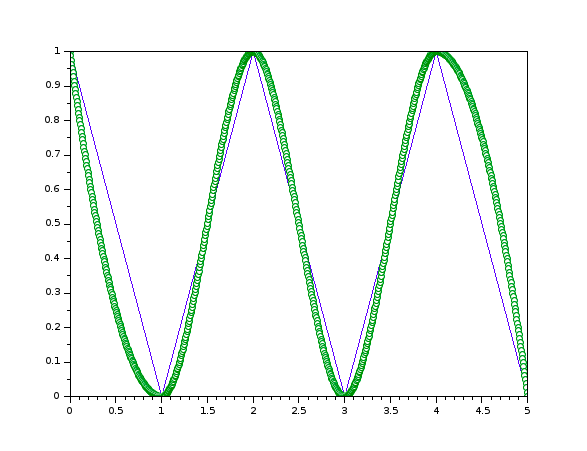
\includegraphics[width = 0.6\textwidth]{pchip.png}
\captionof{figure}{ plot of Interpolation of x and y using PCHIP algorithm}
\label{pchip}
\end{figure}
The figure\ref{pchip} shows the output plot of interpolation using pchip algorithm. \\\\

But there were few functions where we were using the Scilab Octave Interface Toolbox to call few Octave functions. Though we were getting desired output, we were encountering Segmentation-fault (core dumped) issue on exiting the instance. The Scilab instance must essentially exit with a zero, i.e, should exit with exit(0) , for Travis CI to show successful build of the test file. The log was over dumped and was not exiting with exit(0) and the issue we faced is shown below:\\


\begin{figure}[H]
\centering
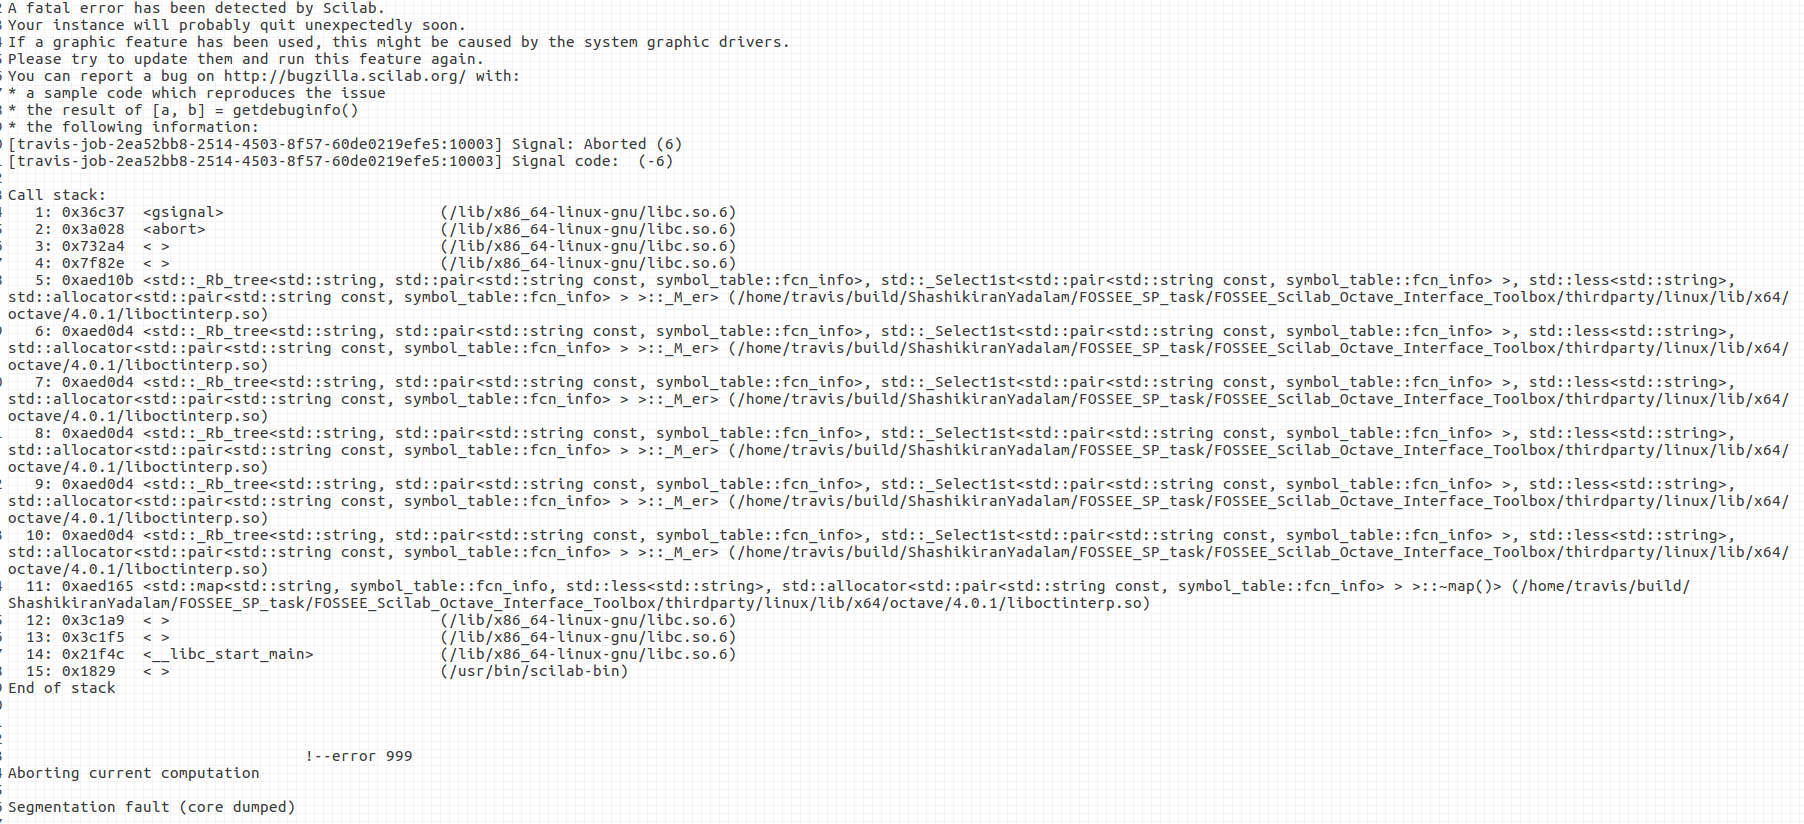
\includegraphics[width = \linewidth]{segfault.png}
\captionof{figure}{ Segmentation fault}
\label{segfault}
\end{figure}
The figure\ref{segfault} shows the segmentation fault issue that we encountered. \\


So after a review by the professor and our mentors, we decided to port the functions which are in Octave Signal package to Scilab. In this process, we encountered few in built functions of Octave, which are not present in Scilab giving the desired output . So we planned, prepared dependency trees and built these function , in a bottom up approach.\\

For example, there is a function called fir1 in the toolbox which is used to implement the FIR filter using window method. This function had fir2 and interp in it which are not there in Scilab. So we built them in Scilab.\\
Also there is another function called residued, which calls for residue which is an inbuilt function in Octave. To build this function in Scilab, we had to build to build five dependencies. The functions mpoles, deconv, polyreduce, polyval and prepad are these dependant functions which are now added to the toolbox.\\




























\chapter{\textbf{Issues faced and Solutions}}
On working on the toolbox, we had faced many issues which we tried to counter them with our own automatations. The issues include :\\

\begin{itemize}
\item GFORTRAN lib issue\\
The version of Scilab that has to be used is Scilab 5.5.2 , to run these toolboxes.\\
We installed Scilab from the official website \url{http://www.scilab.org/download/previous} by choosing Linux OS 64-bit architecture. \\
To load the FOSSEE\textunderscore Scilab\textunderscore Octave\textunderscore Interface\textunderscore toolbox, we had to fix an issue. \\
The library file ‘libgfortran.so.3’ present in the location  \\ \char`\"scilab-5.5.2/lib/thirdparty/redist/  \char`\" 
 had to be moved to the previous directory to load it.This step was important to load the                       FOSSEE\textunderscore Scilab\textunderscore Octave\textunderscore Interface\textunderscore toolbox.

\begin{figure}[H]
\centering
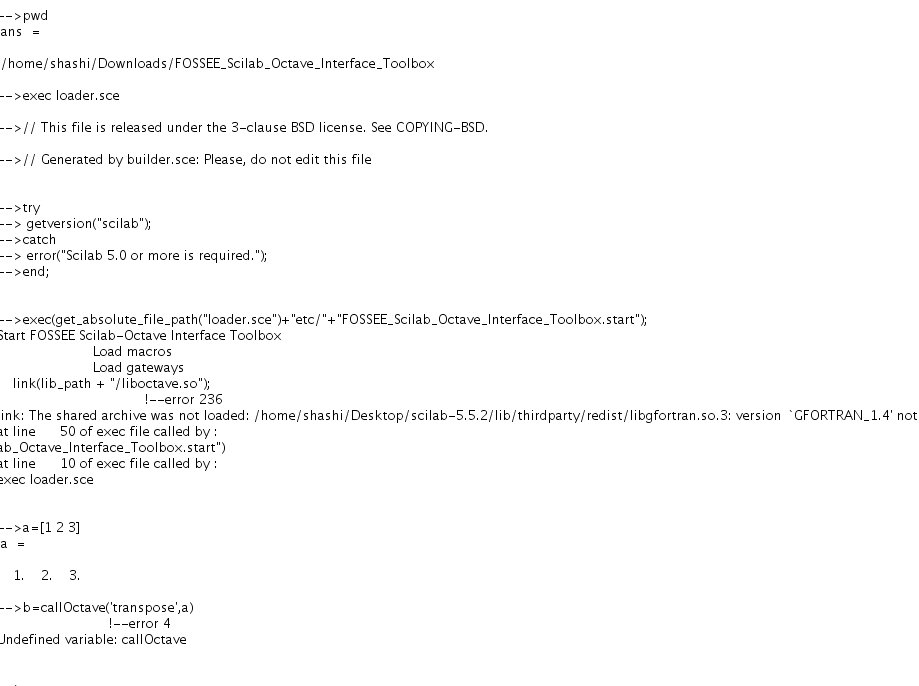
\includegraphics[width = 0.8\textwidth]{gfortran.png}
\captionof{figure}{GFORTRAN 1.4 issue }
\end{figure}

\item The output of few functions were matrices of huge dimensions. These matrices couldn’t be included in the testfile.sce. So we worked on an automation of copying this matrix into a new texfile (if the matrix is square matrix, then we reshaped the matrix by stacking it column wise using command \char`\"matrix \char`\"  ) using the command-\char`\"fprintfMat(\char`\"name\textunderscore of\textunderscore file \char`\" ,desired\textunderscore variable)\char`\" and saved it in macros folder . Then in the the testfile.sce , we scan this text file using the command \char`\" fscanfMat(\char`\"name\textunderscore of\textunderscore file\char`\")\char`\"and store it in dummy variable for comparison.\\

\item Few functions in the toolbox had same names as that of the inbuilt functions. This creates an issue as once the toolbox is built, we could not access the inbuilt functions of scilab. So we changed the names of these functions in the toolbox.The functions include wind.sci and oct\textunderscore interp.sci.


\newpage

\item Also while porting the functions from octave to scilab, we faced an issue regarding the inconsistent operations of vectors. In octave, we can perform addition and subtraction between a row vector and column vector as shown\\


$\begin{bmatrix}
 1&3&4
\end{bmatrix}$-$\begin{bmatrix}
1\\
2\\
3
\end{bmatrix}$=$\begin{bmatrix}
0 & 1 &2 \\
-1 &0  &1 \\
 -2& -1 &0
\end{bmatrix}$ \\

This operation is not possible in scilab and a small operation of such kind in a 350 line code was encountered. We figured out the operation going on in the backend and added that algorithm in to the  corresponding functions. This operation was seen in the function \char`\"residue \char`\".

\item Few functions that had to be ported to scilab ,from octave, had long tree of dependencies,i.e., these functions had inbuilt functions of octave which had to be built in scilab from scratch.(We called it as \char`\"Bottom Up approach\char`\") .




\end{itemize}


\newpage
\title{\textbf{\textbf{\LARGE 
\begin{flushleft}
\textbf{Reference}
\end{flushleft}
}}}




\begin{itemize}
\item \url{https://octave.sourceforge.io/functions_by_package.php}
\item \url{https://octave.org/octave.pdf}
\item  \url{https://in.mathworks.com/help/signal/}
\item \url{ https://in.mathworks.com/help/comm/}
\item \url{ https://en.wikipedia.org/wiki/Window_function}
\end{itemize}
\end{document}



